\begin{frame}
\frametitle{Механические диски (HDD)}
\begin{columns}
  \begin{column}{.6\linewidth}
    \begin{center}
      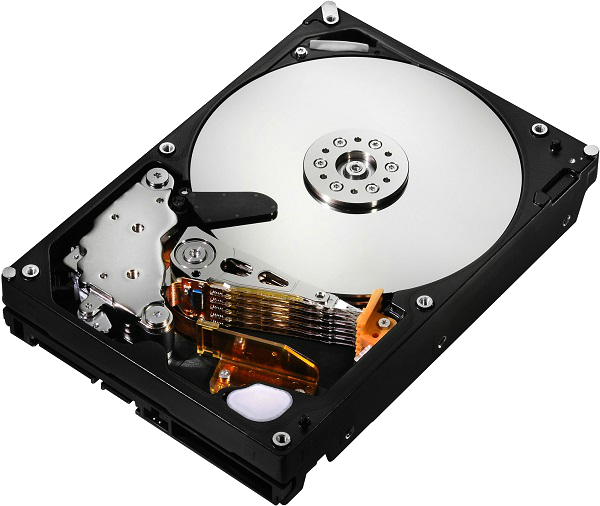
\includegraphics[width=.9\linewidth]{hdd.png}
    \end{center}
  \end{column}
  \begin{column}{.55\linewidth}
    Три основных части:
    \begin{itemize}
      \item вращающиеся диски (platters);
      \item подвижная рука (arm);
      \item читающие/пишушие головы (heads);
    \end{itemize}
  \end{column}
\end{columns}
\end{frame}

\begin{frame}
\frametitle{Скорость HDD}
\begin{itemize}
  \item Скорость вращения дисков HDD:
  \begin{itemize}
    \item при скорости 7200 оборотов в минуту - один оборот 8-9 мс;
    \item чтобы записать/прочитать данные нужно поставить голову над/под нужным
    цилиндром и подождать, пока нужное место диска "доедет" до головы.
  \end{itemize}
  \item Скорость позиционирования читающей/пишушей головы:
  \begin{itemize}
    \item время определяется опять же миллисекундами.
  \end{itemize}
  \item Скорость работы диска доминируется поиском:
  \begin{itemize}
    \item скорость вращения диска + позиционирование головы;
    \item random IO гораздо медленнее sequential IO.
  \end{itemize}
\end{itemize}
\end{frame}

\begin{frame}
\frametitle{Скорость HDD}
\begin{center}
  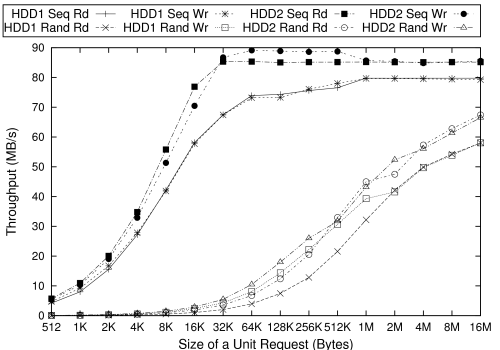
\includegraphics[width=.8\linewidth]{hdd_perf.png}
\end{center}
\end{frame}
